\chapter{Completeness analysis}
\label{chapter:cad}

\begin{table}
\caption{ \smr\ Level1B and Level2 data count by frequency mode.}
\label{table:count}
\scalebox{0.965}{%
\begin{tabular}{|l|l|l|l|}
  \hline
  \textbf{Frequency mode} & \textbf{Level1B count} & \textbf{Level2 count}  & \textbf{Fraction [\(\%\)]} \\
  \hline
  \hline
  01 & 1924043 & 1711616 & 89.0\\
  \hline
  \hline
  02 & to be filled in & - & - \\
  \hline
  \hline
  08 & 400901 & 335727 & 83.7\\
  \hline
  \hline
  13 & 356987 & 294608 & 82.5\\
  \hline
  \hline
  14 & 365195 & 218611 & 59.9\\
  \hline
  \hline
  19 & 397295 & 331308 & 83.4\\
  \hline
  \hline
  21 & 344476 & 299992 & 87.1 \\
  \hline
  \hline
  22 & 93374 & 56768 & 60.8 \\
  \hline
  \hline
  24 & 15794 & 12873 & 81.5 \\
  \hline
\end{tabular}}
\end{table}


Table~\ref{table:count} and Figure~\ref{fig:l2cad-fm1} to Figure~\ref{fig:l2cad-fm24}
show the amount af available Level1B data and succesfully
processed Level2 data for the considered FreqModes and
for the complete mission and by month.
The amount of available Level1B data varies during mission,
and there are a number of reasons for this.
During the first six years of the mission \smr\ was operated
both in aeronomy and astronomy mode, and hence less
aeronomy observations are available for these years
compared to after 2008.  
During the most recent years \smr\ has both partly and completely
been turned off during the summer month.
\smr\ is a flexible instrument, as described in Sect.~\ref{sec:odin}
but, in prinicipal, only two frequency modes (FreqModes)
can be applied at a given time. The observation program, or how
often the various FreqModes are used, has been varied during the
mission.

FreqMode 1 and 2 (not yet fully processed and Figure is missing)
are the most frequently applied modes, and 5000-10000 scans have been
observed each month. Level2 processing have been succesfully
for the majority (89\,\%) of the available Level1B data.
One of the main reason for an unsuccesful Level2 processing is here
that some scans do not cover a required altitude range, 
i.e. not enough spread of the tangent altitude of individual spectra. 

Level2 processing of the FreqMode 21 (\chem{NO} mode) have also
a relatively high succes rate (87\,\%).
For the water vapor modes around 557 GHz (FreqMode
13 and 19) the succes rate is around 83\,\%.
 


FreqMode 14, 22, 24 are deployed for \chem{CO} observations.
The frontend used for these observations have been unstable
(drifting in frequency), and that can result in that the 
\chem{CO} signature is not covered in observed spectra 
of some of the scans. This gives that the fraction of
sussessful level2 processing is lower for these modes
compared to the others.
 
More text here...




\begin{figure}[t]
\centering
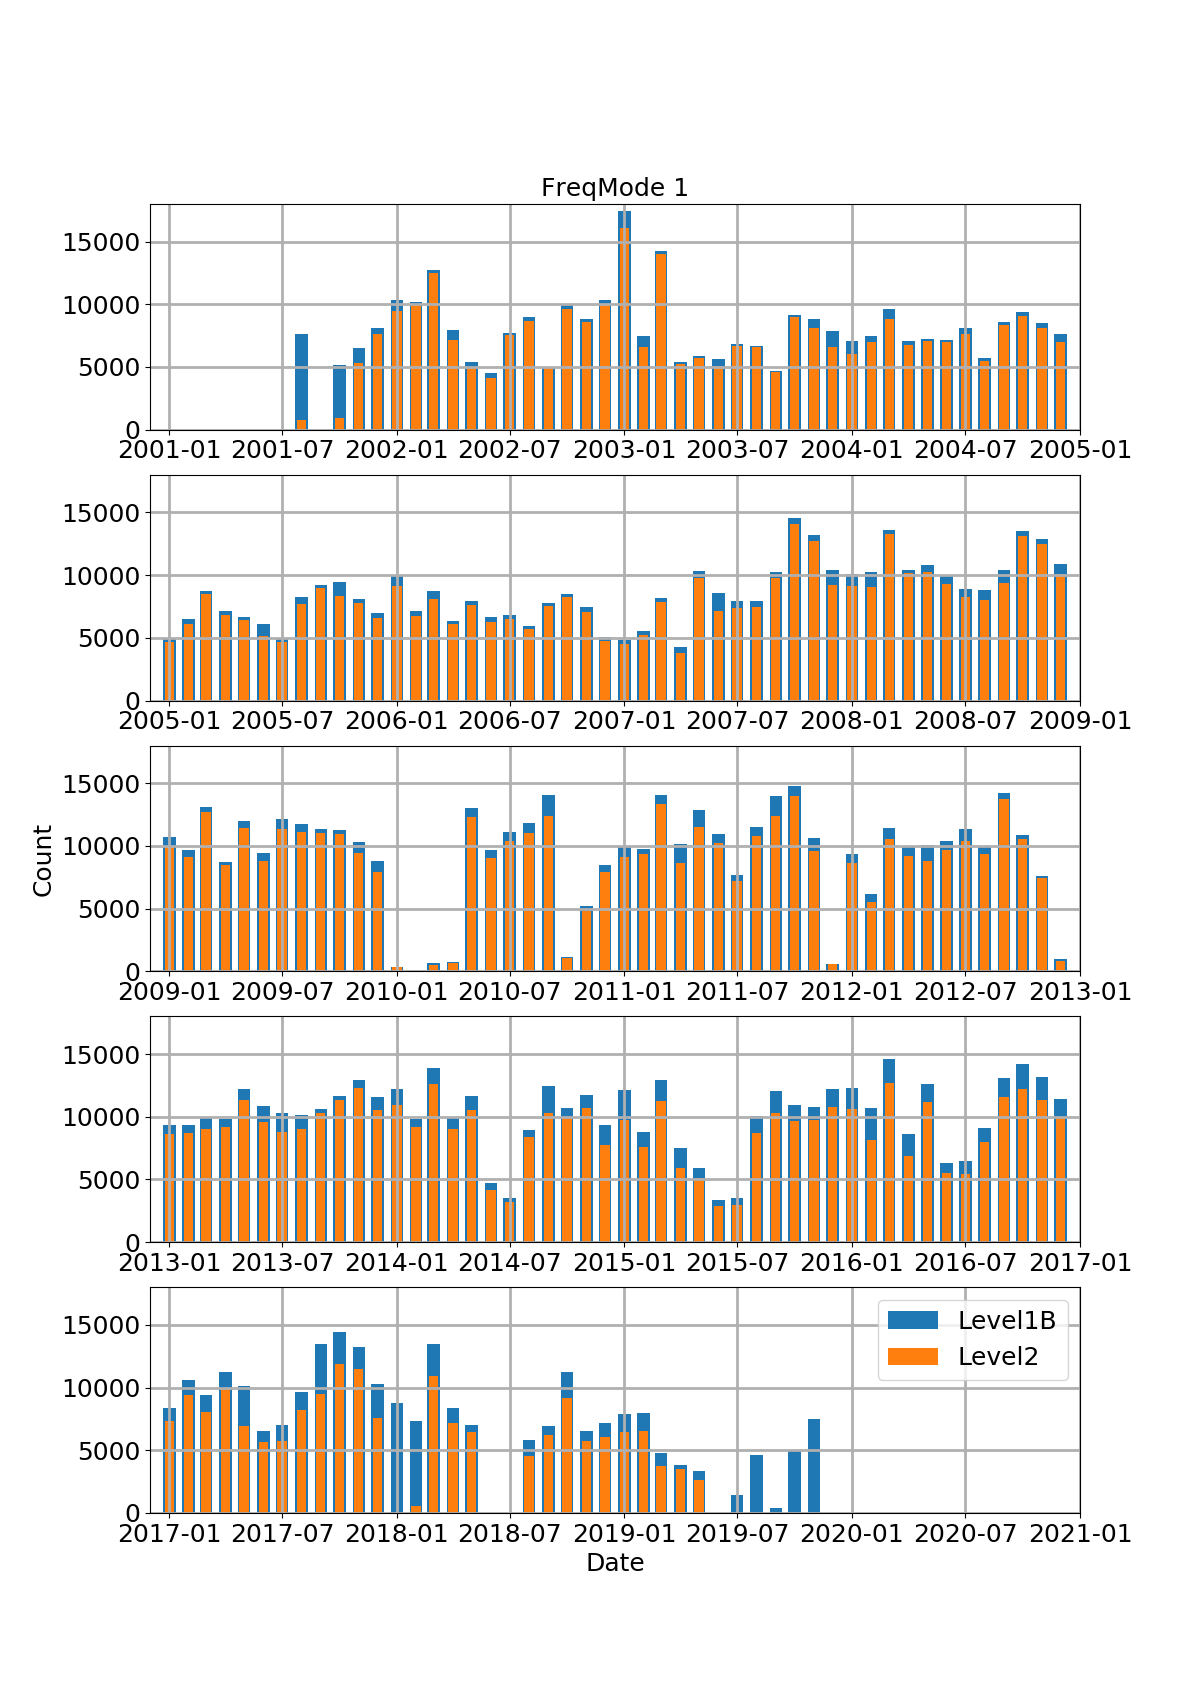
\includegraphics[width=1.0\textwidth]{l2cad-fm1.png}
\caption{Number of available Level1b and succesfully processed Level2
scans by month for FreqMode 1, during the complete \smr\ mission.}
\label{fig:l2cad-fm1}
\end{figure}

\begin{figure}[t]
\centering
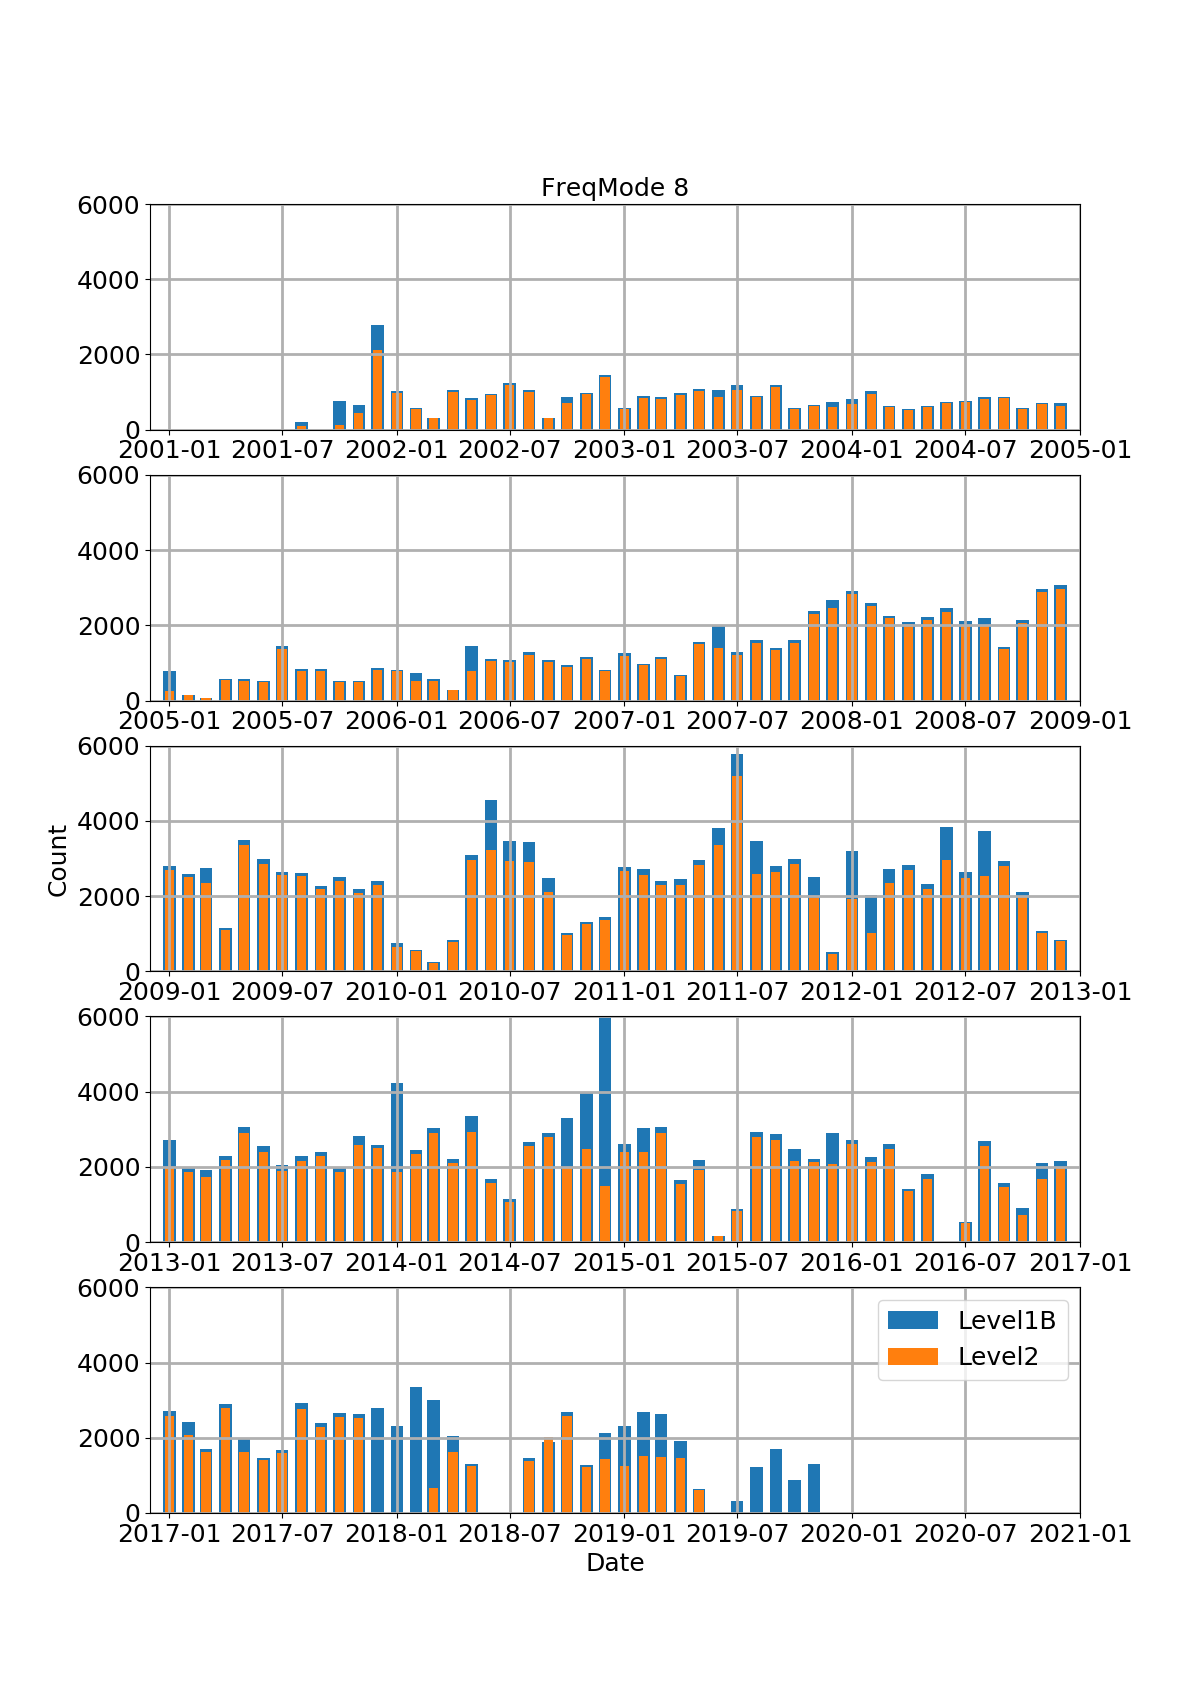
\includegraphics[width=1.0\textwidth]{l2cad-fm8.png}
\caption{As Figure~\ref{fig:l2cad-fm1} but for FreqMode 8.}
\label{fig:l2cad-fm8}
\end{figure}

\begin{figure}[t]
\centering
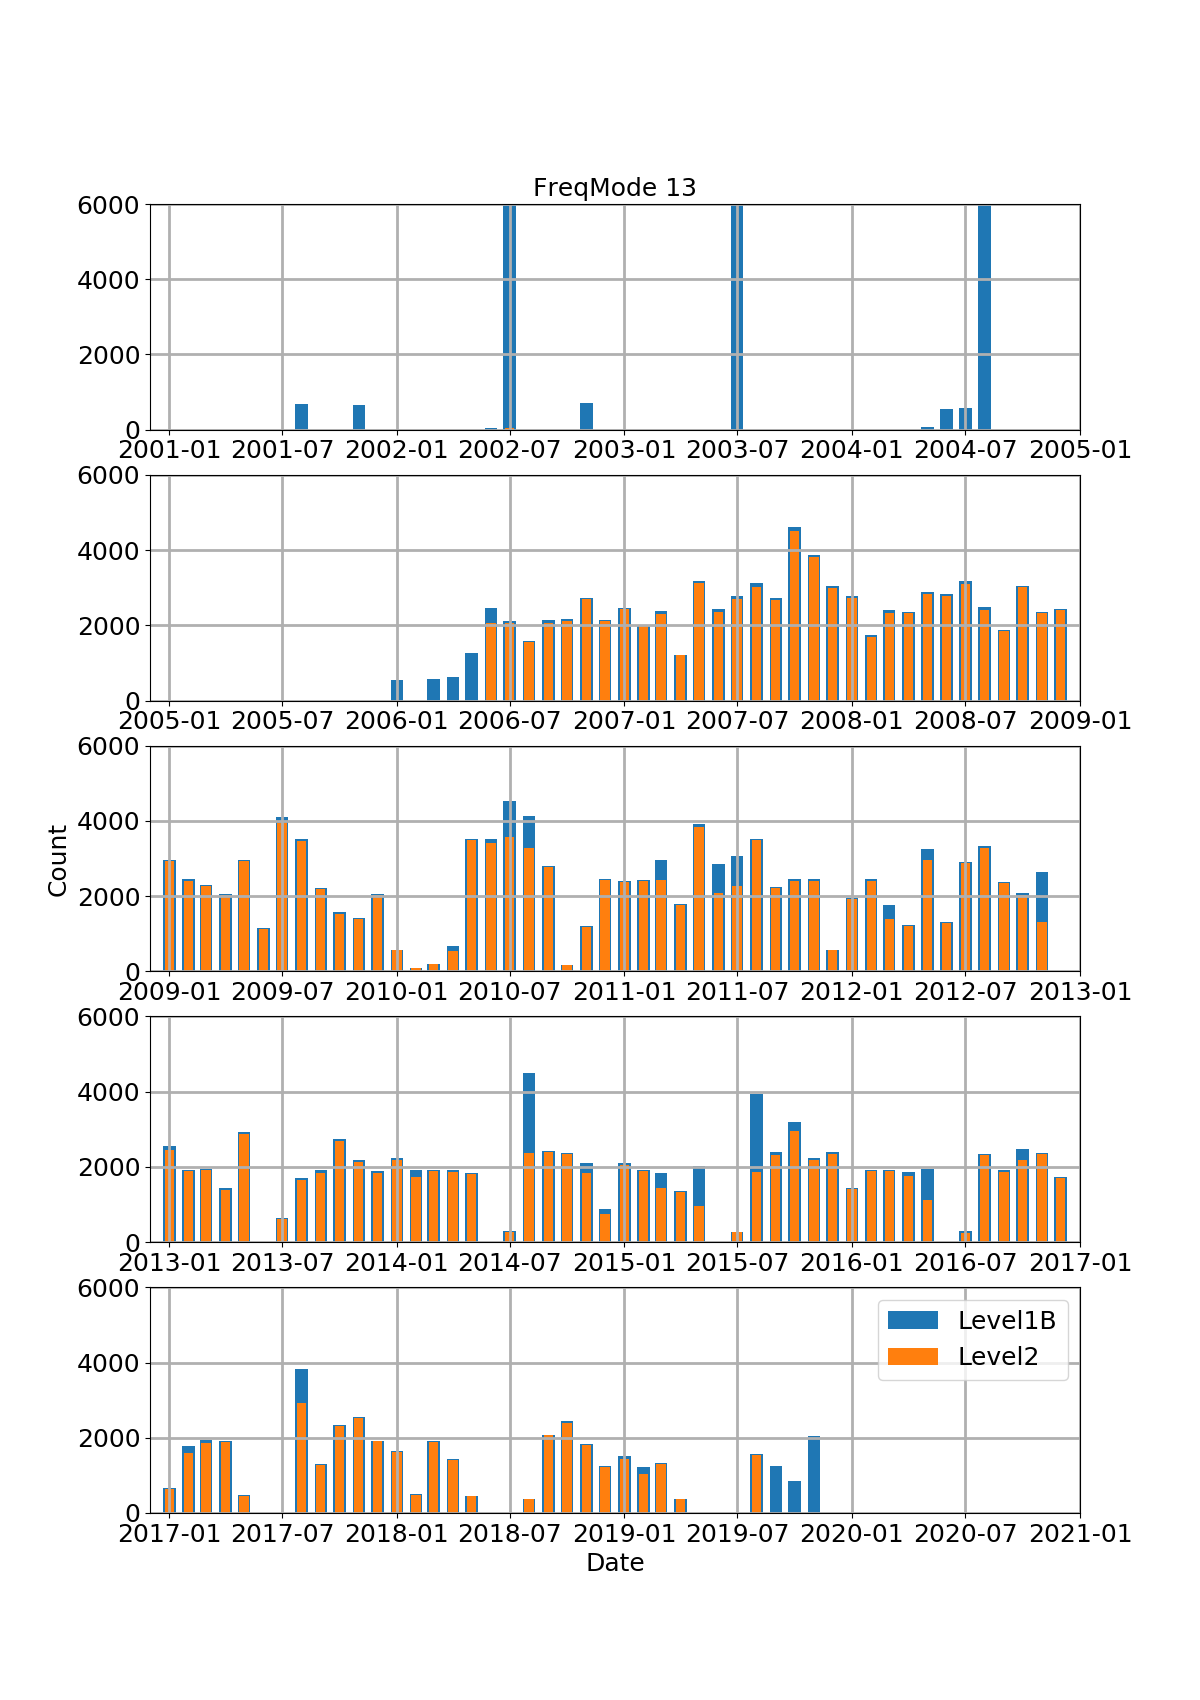
\includegraphics[width=1.0\textwidth]{l2cad-fm13.png}
\caption{As Figure~\ref{fig:l2cad-fm1} but for FreqMode 13.}
\label{fig:l2cad-fm13}
\end{figure}

\begin{figure}[t]
\centering
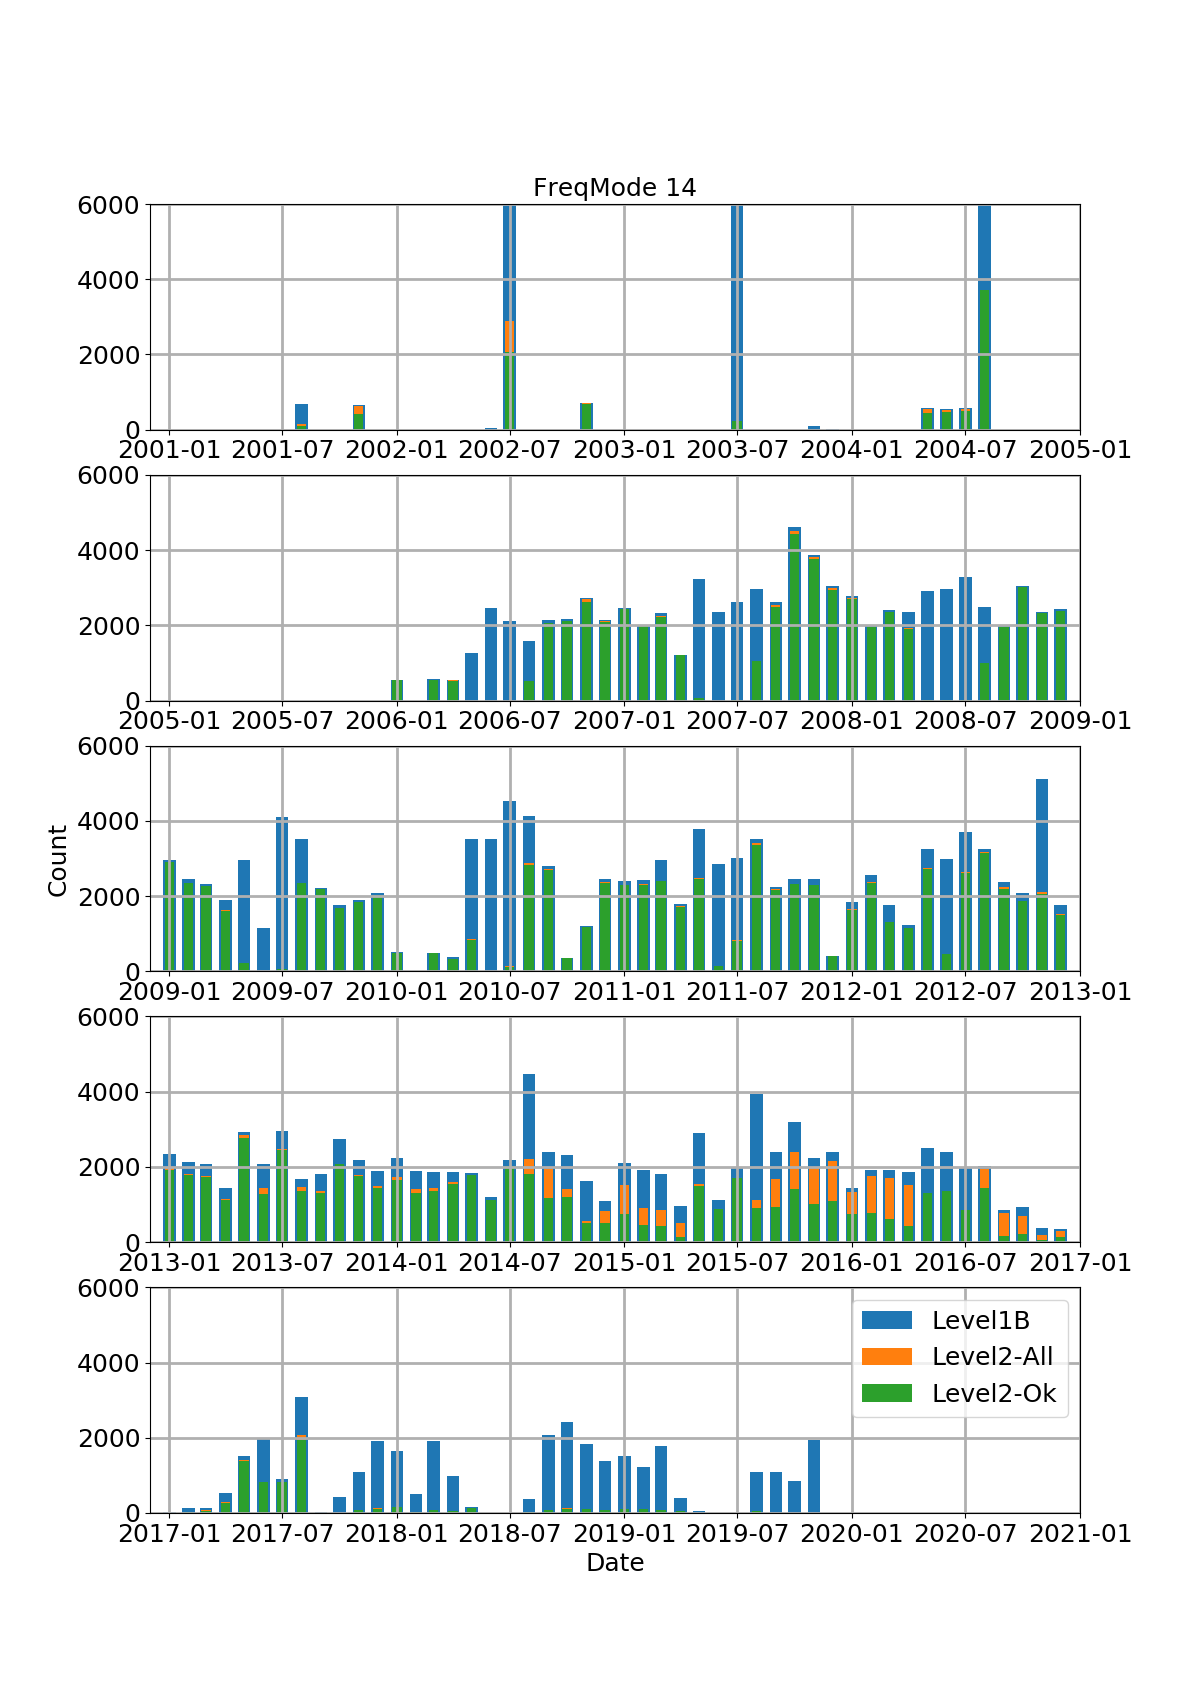
\includegraphics[width=1.0\textwidth]{l2cad-fm14.png}
\caption{As Figure~\ref{fig:l2cad-fm1} but for FreqMode 14.}
\label{fig:l2cad-fm14}
\end{figure}

\begin{figure}[t]
\centering
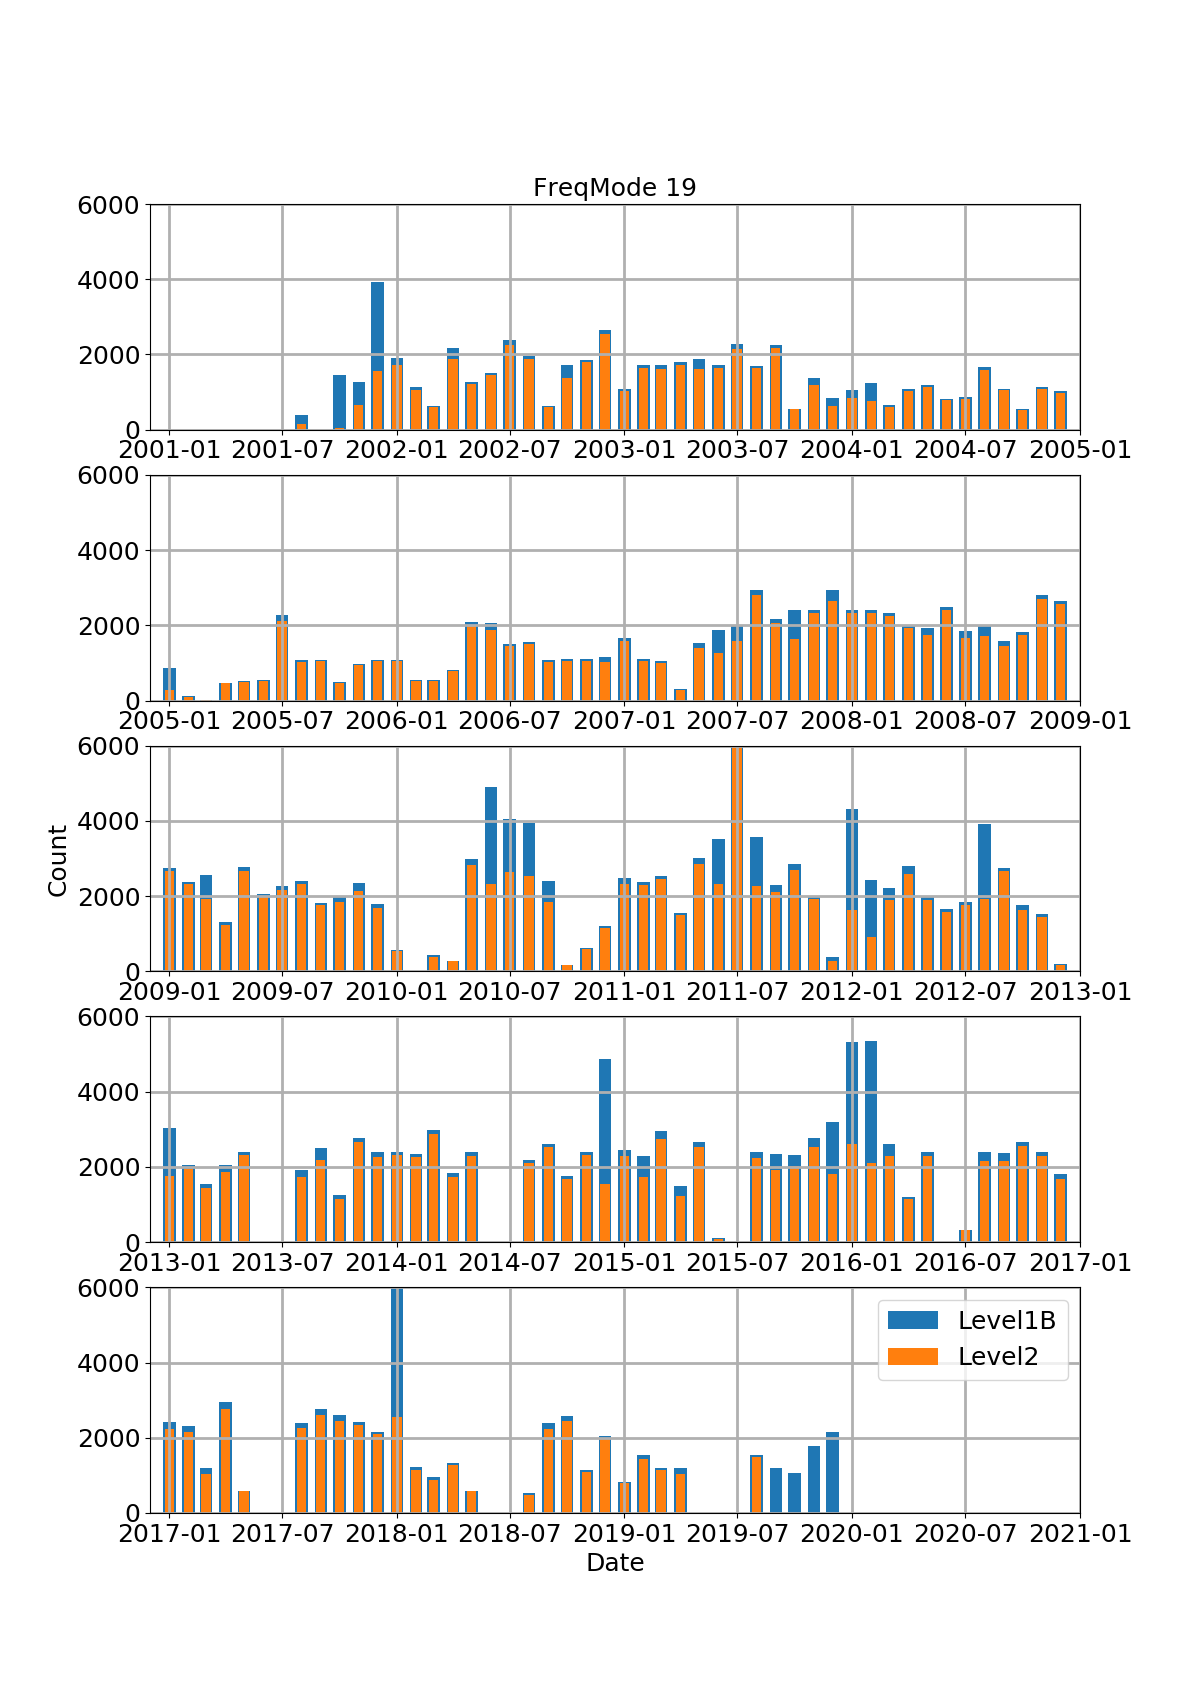
\includegraphics[width=1.0\textwidth]{l2cad-fm19.png}
\caption{As Figure~\ref{fig:l2cad-fm1} but for FreqMode 19.}
\label{fig:l2cad-fm19}
\end{figure}

\begin{figure}[t]
\centering
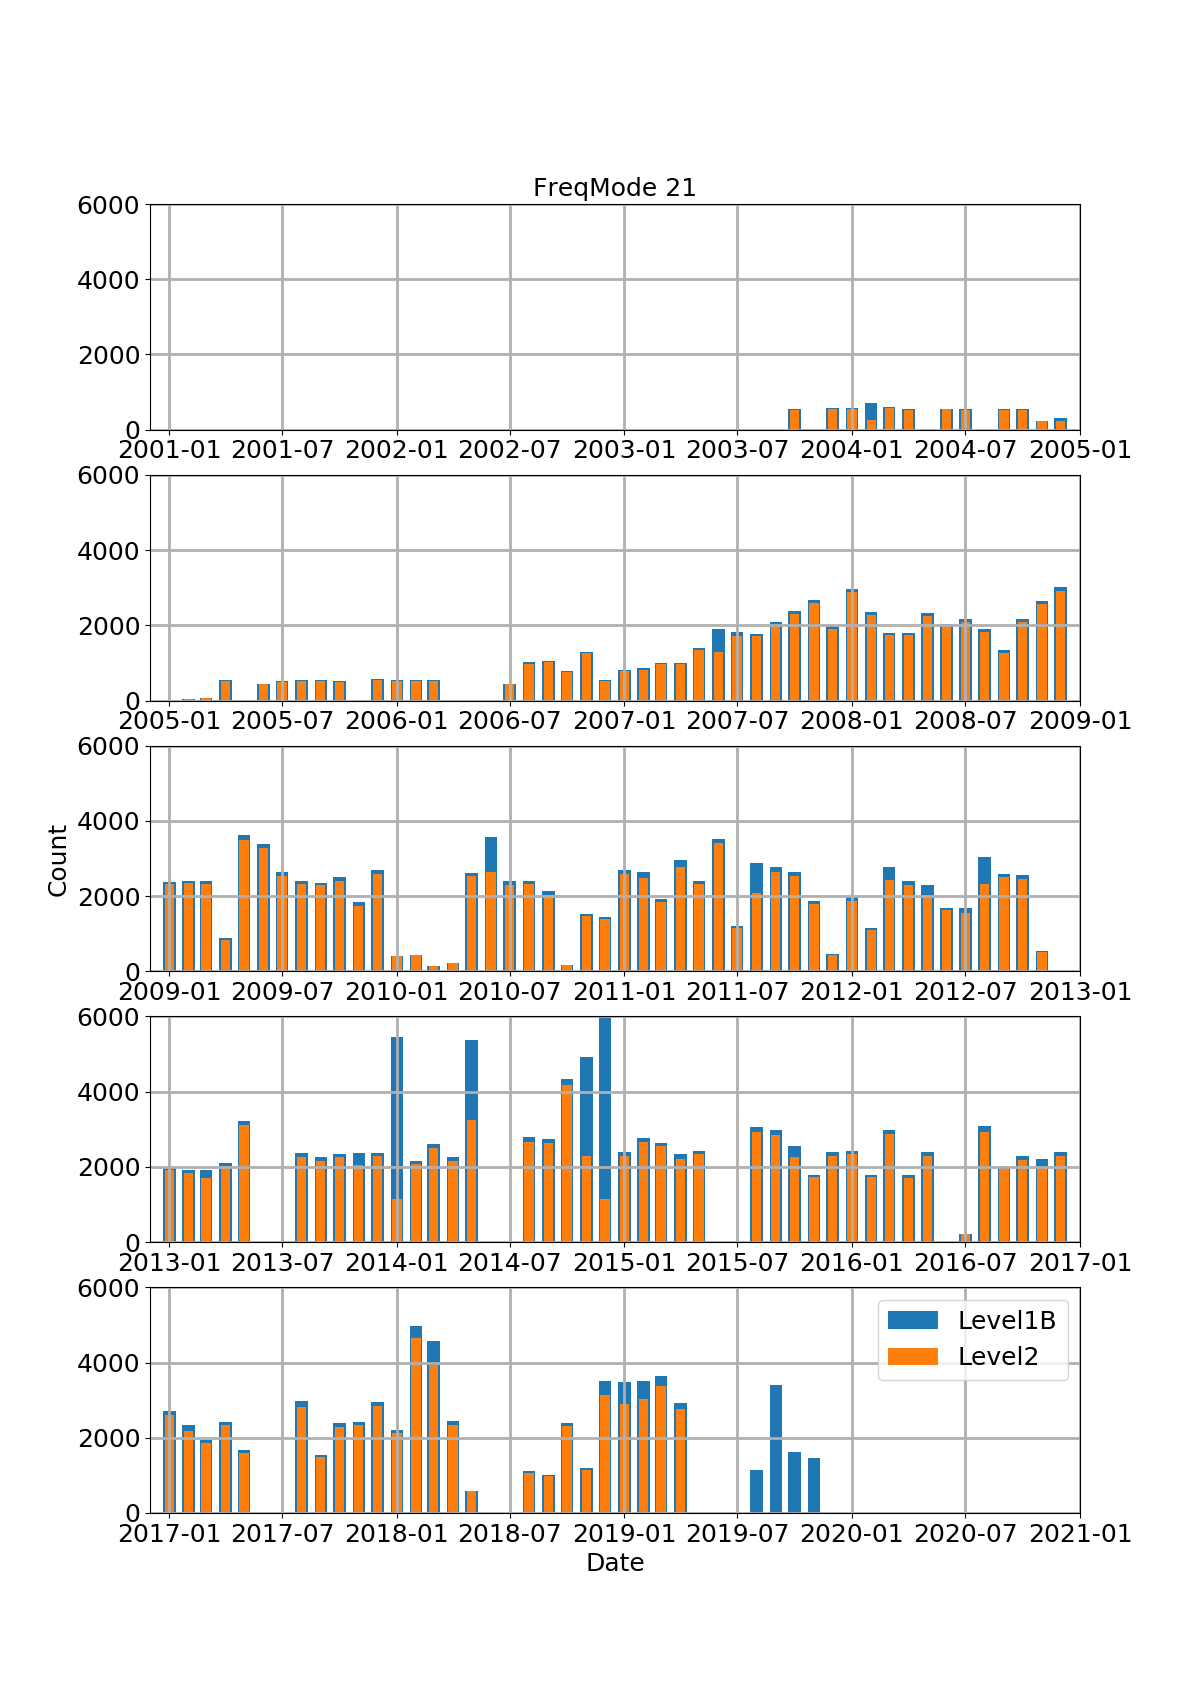
\includegraphics[width=1.0\textwidth]{l2cad-fm21.png}
\caption{As Figure~\ref{fig:l2cad-fm1} but for FreqMode 21.}
\label{fig:l2cad-fm21}
\end{figure}

\begin{figure}[t]
\centering
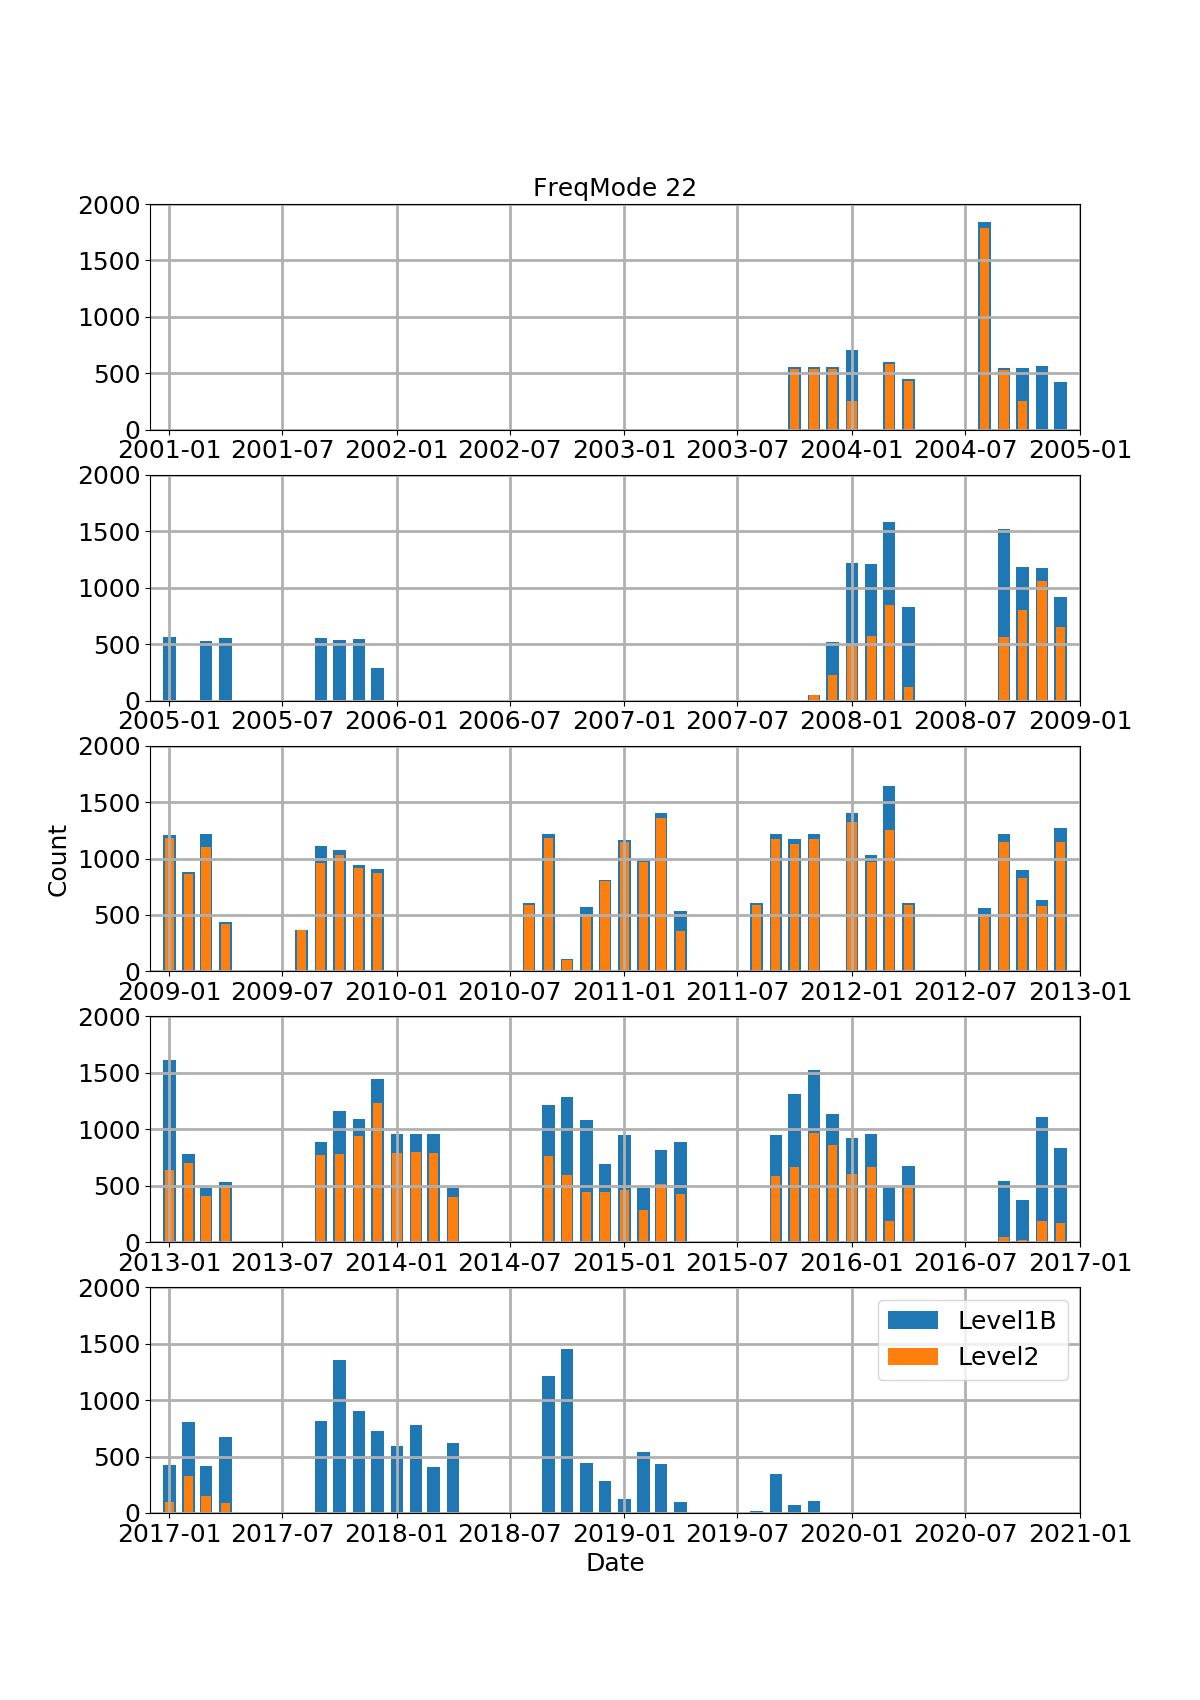
\includegraphics[width=1.0\textwidth]{l2cad-fm22.png}
\caption{As Figure~\ref{fig:l2cad-fm1} but for FreqMode 22.}
\label{fig:l2cad-fm22}
\end{figure}

\begin{figure}[t]
\centering
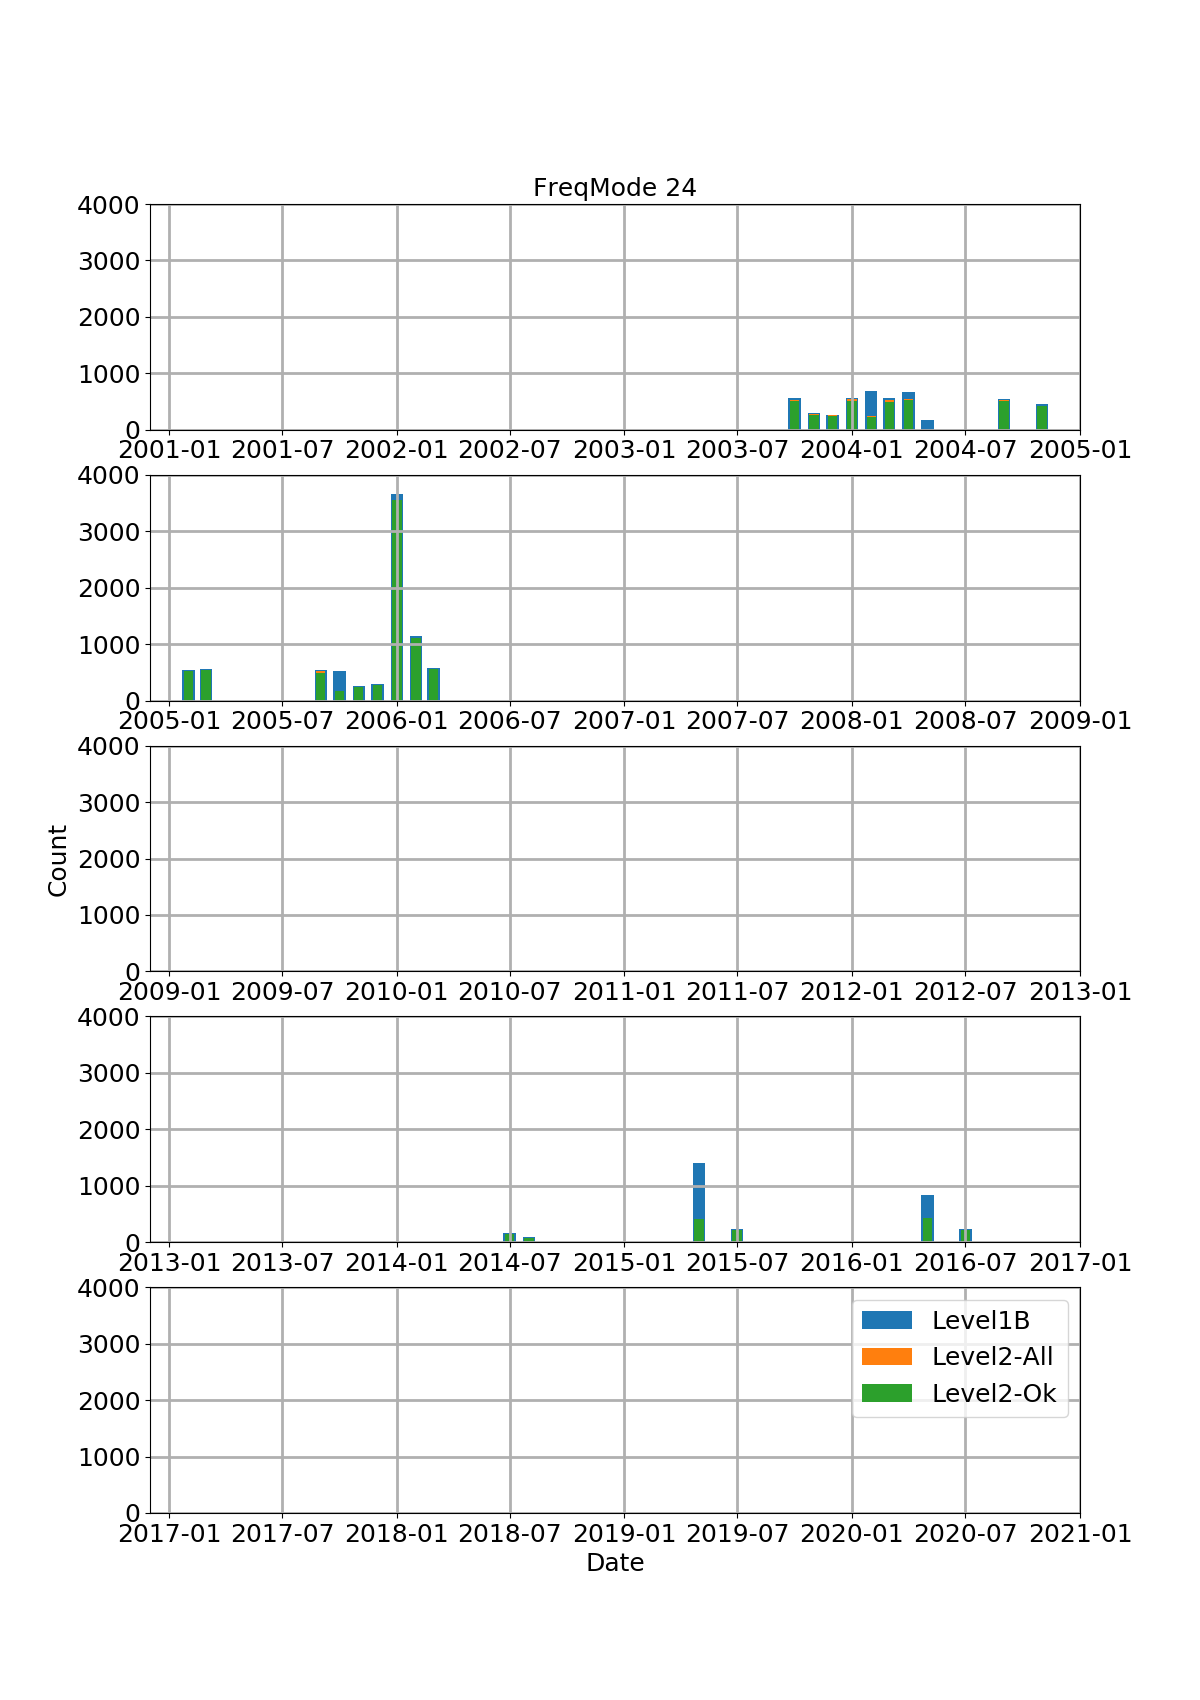
\includegraphics[width=1.0\textwidth]{l2cad-fm24.png}
\caption{As Figure~\ref{fig:l2cad-fm1} but for FreqMode 24.}
\label{fig:l2cad-fm24}
\end{figure}
